\documentclass[11pt,hyperref={bookmarks=false}]{beamer}
\usetheme{Warsaw}
%\usetheme{Madrid}
%\usecolortheme{beaver}
\usefonttheme{professionalfonts}
 \usepackage[usenames,dvipsnames]{pstricks}
 \usepackage{wallpaper}
 \usepackage{epsfig}
\definecolor{UniBlue}{RGB}{157,34,53}
\setbeamercolor{block title}{bg=UniBlue!70,fg=black}

\usepackage{psfrag,graphicx}
\usepackage{amsmath,amsfonts}
\usepackage{lscape}
\usepackage{array,epsfig}
\usepackage{amsfonts}
\usepackage{amssymb}
\usepackage{amsxtra}
\usepackage{amsthm}
\usepackage{makecell}
\usepackage[skip=0pt, belowskip=-10pt]{caption}
\usepackage{subcaption}
\usepackage{float}
\usepackage{multirow}
\usepackage{booktabs}
%\usepackage{subfigure}
\usepackage{eso-pic}
\usepackage{transparent}
\usepackage{graphicx}
\usepackage{tikz}
\usepackage{longtable}
\newtheorem{df}{Definition}
\newtheorem{lm}{Lemma}
\newtheorem{prp}{Proposition}
\newtheorem{sprf}{Sketch of Proof}
\newtheorem{prf}{Proof}
\newtheorem{conjecture}{Conjecture}
\newtheorem{suffc}{Sufficient Condition}
\setbeameroption{hide notes}
\newcommand{\threelinebracer}{$\left. \begin{array}{c} \\ \\ \\ \end{array} \right\rbrace$}
\newcommand{\threelinebracel}{$\left. \begin{array}{c} \\ \\ \\ \end{array} \right\lbrace$}
\newcommand{\twolinebracer}{$\left. \begin{array}{c} \\ \\ \end{array} \right\rbrace$}
\newcommand{\twolinebracel}{$\left. \begin{array}{c} \\ \\ \end{array} \right\lbrace$}
\newcommand{\bd}{\partial}
\usepackage{threeparttable}
\usepackage{pgf}  
%\logo{\pgfputat{\pgfxy(-1.2,-0.2)}{\pgfbox[center,base]{\includegraphics[height=12pt, keepaspectratio]{UA_Logo_Horizontal.eps}}} }

%\usebackgroundtemplate
%{
  %  \node[opacity=0.3, at=(current page.south east),anchor=south east,inner sep=0pt] 
    %\includegraphics[width=\paperwidth,height=20pt]{UA_Logo_Horizontal.eps}%
%}

\linespread{1}
\usepackage{parskip}
%\setlength{\itemsep}{1em} 
%\addtolength{\parskip}{5pt}
\DeclareMathSizes{12}{10}{8}{6}
%  \begin{itemize}}{\end{itemize}}
% Separate slides by \begin{frame} and \end{frame}.
\title[Willingness-to-pay for Warnings]{Willingness-to-pay for Warnings}
\author[A. Gaduh, P. McGee and A. Ugarov]{A. Gaduh, P. McGee and A. Ugarov}
\institute[]{}
\date{\today}


\begin{document}
%\AddToShipoutPicture*{\BackgroundPic}

\begin{frame}
\titlepage
\end{frame}

%%%%%%%%%%%%%%%%%%%%%%%%%%%%%%%%%%%%%%%%%%%%%%%%%%%%%%%%%%%%%%%%%%%%%%%%%%%%%%%%%%%%%%%%%%%%%%%%
%%%%%%%%%%%%%%%%%%%%%%%%%%%%%%%%%%%%%%%%%%%%%%%%%%%%%%%%%%%%%%%%%%%%%%%%%%%%%%%%%%%%%%%%%%%%%%%%



\begin{frame}
\frametitle{Motivation}
\begin{itemize}
\item Many real-life situations require alarm designers to determine risk thresholds for sounding alarms: medical tests, fire alarms, extreme weather warnings, etc
\item This requires balancing the costs of false-positive and false-negative events
\item There is little theory and even less empirical studies on people preferences over signal characteristics
\end{itemize}
\end{frame}



\begin{frame}
\frametitle{Research Questions}
\begin{enumerate}
\item How do signal characteristics affect protective response?
\item Which signal characteristics people prefer? Two hypotheses:
\begin{itemize}
\item Risk-neutral decision model provides a good description of user's preferences
\item Subjects put equal weights on costs coming from false-positive and false-negative events
\end{itemize}
\end{enumerate}
\end{frame}



\begin{frame}
\frametitle{Findings}
\begin{itemize}
\item There are significant deviations from the risk-neutral model both for protective decisions and for willingness-to-pay for signals
\item WTP has excess sensitivity to false-negative rates for low priors, and lower sensitivity for high priors (vice versa for false-positive)
\item Subjects tend to have excessive reactions to false-positive rates with negative signals and excessive reactions to false-negative rates for positive signals (alarms)
\item This effect partially comes from distorted beliefs on posterior chances of false-positive/false-negative event conditional on a signal
\item This patter is not consistent with EU framework, but most consistent with decision-making heuristic in which subjects do not differentiate between false-positive and false-negative rates when choosing signals
\end{itemize}
\end{frame}


\begin{frame}
\frametitle{Overview of the Experiment}
\framesubtitle{Willingness to pay (WTP) for signals}
\begin{itemize}
	\item An insurance experiment:
		\begin{itemize}
			\item Two states of the world: bad ($\omega=1$) and good ($\omega=0$)
			\item Probability of a bad state is $P (\omega=1) = \pi$
			\item Bad state $\implies$ loss of \$$L$
			\item A perfectly protective insurance can be purchased for \$$c$
		\end{itemize}
	\item Subject can purchase a signal $s$ before purchasing the insurance:
		\begin{itemize}
			\item A signal is characterized by its true-positive ($P(s=1|\omega=1)$) and true-negative rates ($P(s=0|\omega=0)$) 
		\end{itemize}
\end{itemize}
\end{frame}


\begin{frame}
\frametitle{WTP for Signals}
\framesubtitle{Theory}

\begin{itemize}
	\item Theoretically, what should be the WTP for a signal?
	\item If bad states are a priori rare ($\pi L<<c$) $\implies$ never protect without a signal
	\item The theoretical WTP $b$ for an expected utility maximizer given a signal $s$ is a solution $b^*$ to the following:
	\[
	\small
	\begin{split}
		P(s=1) &u(Y_0-b^*-c) + \pi P(s=0|\omega=1)u(Y_0-b^*-L)+\\ 
		&+(1-\pi)P(s=0|\omega=0)u(Y_0-b^*) =\\
		&=(1-\pi)u(Y_0)+\pi u(Y_0-L)
	\end{split}
	\]
	\normalsize
	\item A risk-neutral agent would therefore pay:
		\[b^*=\pi(1-P(s=0|\omega=1))L-P(s=1)c\]
\end{itemize}
\end{frame}

\begin{frame}
\frametitle{Experiment Basics}
\begin{enumerate}
\item Box with 20 white and black balls (black ball=bad state)
\item Assumptions:
\begin{itemize}
\item Protection cost is \$5
\item Loss without protection is \$20
\item Cost-loss ratio is $c/L=5/20=0.25$
\end{itemize}
\item Signal is an unreliable hint about the ball color
\item Vary the prior probability of bad state and the signal's information structure
\end{enumerate}
\end{frame}


\begin{frame}
\frametitle{Representing Signals}
\begin{itemize}
\item A subject receives a noisy signal as a hint from one of the gremlins:
\end{itemize}
\begin{center}
\newcolumntype{C}{ >{\centering\arraybackslash} m{2cm} }
%\newcolumntype{L}{ >{\left\arraybackslash} m{4cm} }

\small
\begin{tabular}{l|C|C|C|C}
\hline
Ball/Gremlin & 
\includegraphics[width=0.15\textwidth]{Instructions/honest.png} &  
\includegraphics[width=0.15\textwidth]{Instructions/whiteswamp.png} &  
\includegraphics[width=0.15\textwidth]{Instructions/blackswamp.png} \\
 \hline
  &  & &  \\

\includegraphics[width=0.1\textwidth]{Instructions/whiteball.png}  & The Ball is white! \vspace{10pt} &The Ball is white! \vspace{10pt} & The Ball is black! \vspace{10pt}\\
\hline
  &  & &  \\

\includegraphics[width=0.1\textwidth]{Instructions/blackball.png}  & The Ball is black! \vspace{10pt} & The Ball is white! \vspace{10pt}& The Ball is black! \vspace{10pt} \\
\hline
\end{tabular}
\end{center}
\end{frame}


\begin{frame}
\frametitle{Experiment Progression}
\begin{enumerate}
\item \textbf{Blind Protection Game:} Protection response conditional on prior probability
\item \textbf{Informed Protection Game:} Protection response conditional on prior probability and signal
\item \textbf{Belief Elicitation:} Subjects beliefs about the bad state's probability conditional on prior and signal
\item \textbf{WTP Elicitation:} Willingness-to-pay for each signal
\end{enumerate}
\end{frame}


\begin{frame}
\frametitle{Going over all the treatments}
\begin{itemize}
\item Out of 4 tasks, two are novel (informed protection and WTP elicitation for a signal)
\item We report basic results to show that the subjects' behavior is largely sensible in all the tasks
\item Responses demonstrate known biases in existing tasks
\end{itemize}
\end{frame}



\begin{frame}
\frametitle{Blind Protection (No Signal)}
\begin{columns}
\begin{column}{0.5\textwidth}
\begin{itemize}
\item There is more protection when the probability of black ball is higher
\item Responses are mostly monotonic in probability
\item There are both risk-averse and risk-loving subjects
\end{itemize}
\end{column}

\begin{column}{0.5\textwidth}
\begin{center}
%\begin{figure}
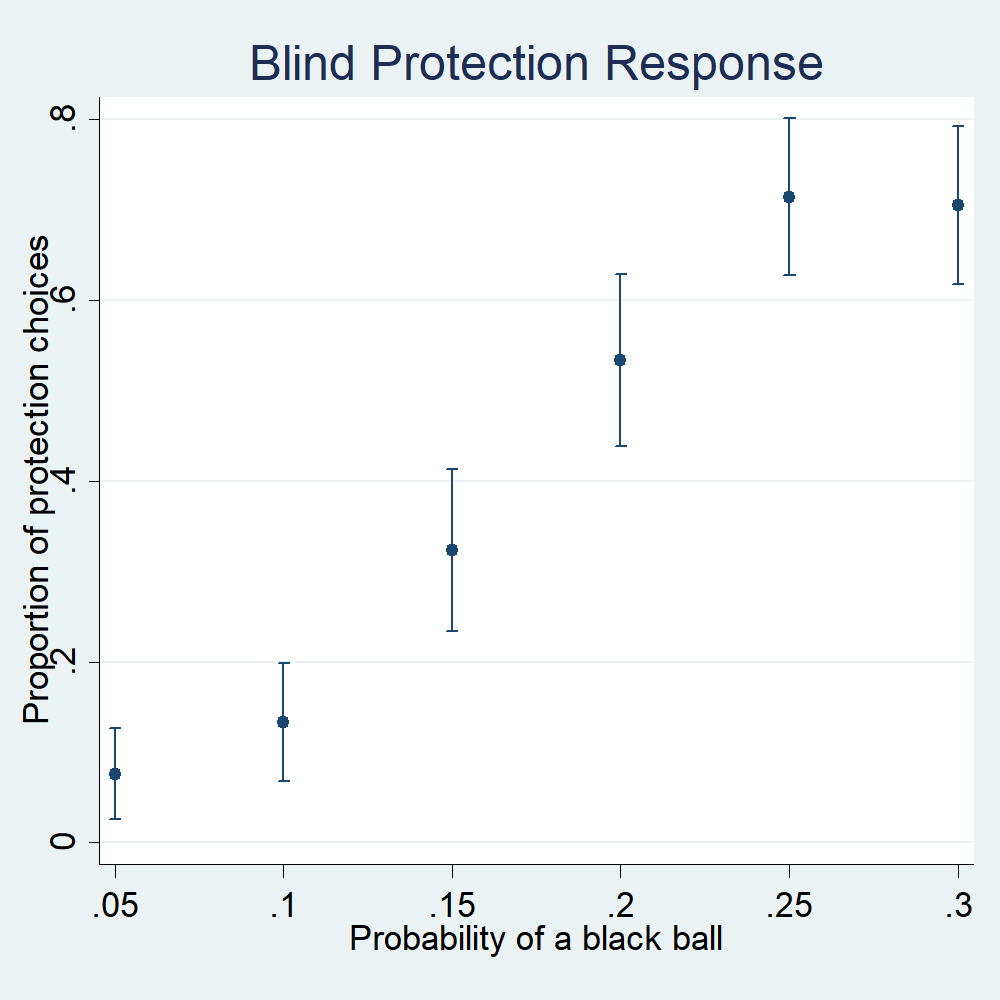
\includegraphics[width=\textwidth]{Graphs/blind_prot_sta.png}
%\end{figure}
\end{center}
\end{column}
\end{columns}
\end{frame}




\begin{frame}
\frametitle{Informed Protection}
\begin{itemize}
\item Protection rates increase with the posterior probability of a bad event (black ball)
\item Average protection probability is no longer monotonic in posteriors due to lower N of obs per prob and due to posterior estimation mistakes 
\end{itemize}
\begin{figure}[h]
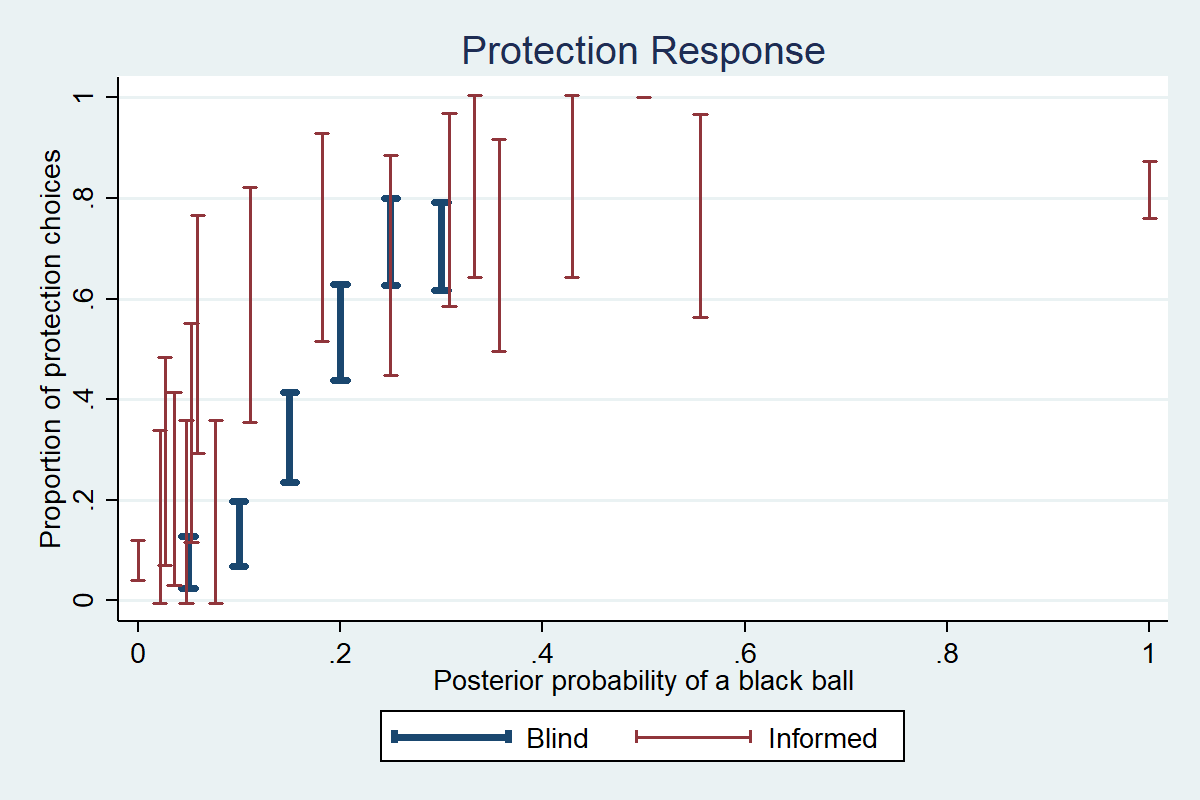
\includegraphics[scale=0.15]{Graphs/ip_response_comp.png}
\end{figure}
\end{frame}




\begin{frame}
\frametitle{IP Big Picture}
\begin{itemize}
\item Overprotect in response to white signals, underprotect in response to black signals without false-positive: can be explained by risk preferences
\item Overprotect in response to white signals with FP (cannot be explained by risk preferences)!
\end{itemize}
\scriptsize
\begin{table}[H]\centering \scriptsize \begin{tabular}{ccccccc} \hline \hline
\textbf{Signal}&\textbf{False-pos.}&\textbf{False-neg.}&\textbf{\% protect}& \textbf{Posterior} & \textbf{Optimal} & \textbf{P(=optimal)} \\ \hline
White&No&No&0.000&0.067&0.000&0.000\\
White&No&Yes&0.100&0.333&0.000&0.000\\
White&Yes&No&0.000&0.130&0.000&0.000\\
White&Yes&Yes&0.131&0.564&0.121&0.000\\
Black&No&No&1.000&0.846&1.000&0.000\\
Black&No&Yes&1.000&0.841&1.000&0.000\\
Black&Yes&No&0.550&0.833&0.870&0.355\\
Black&Yes&Yes&0.483&0.886&0.871&0.685\\
\hline \end{tabular} \end{table}

\end{frame}



\begin{frame}
\frametitle{Belief Elicitation}
\begin{columns}
\begin{column}{0.5\textwidth}
\begin{itemize}
\item Correlation between beliefs and posteriors
\item Large dispersion of errors
\item Includes surprisingly large errors even for certain signals
\end{itemize}
\end{column}

\begin{column}{0.5\textwidth}
\begin{center}
\begin{figure}
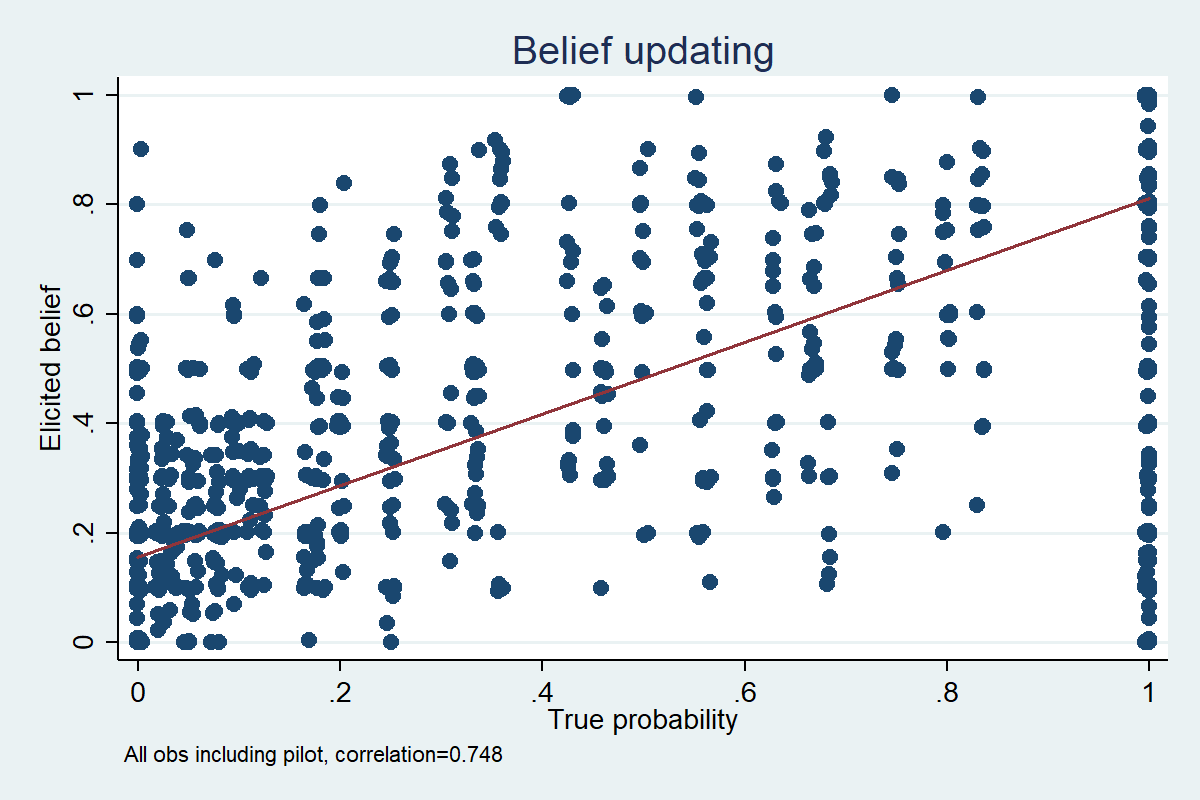
\includegraphics[width=0.9\textwidth]{Graphs/updating_s1.png}
\end{figure}
\begin{figure}
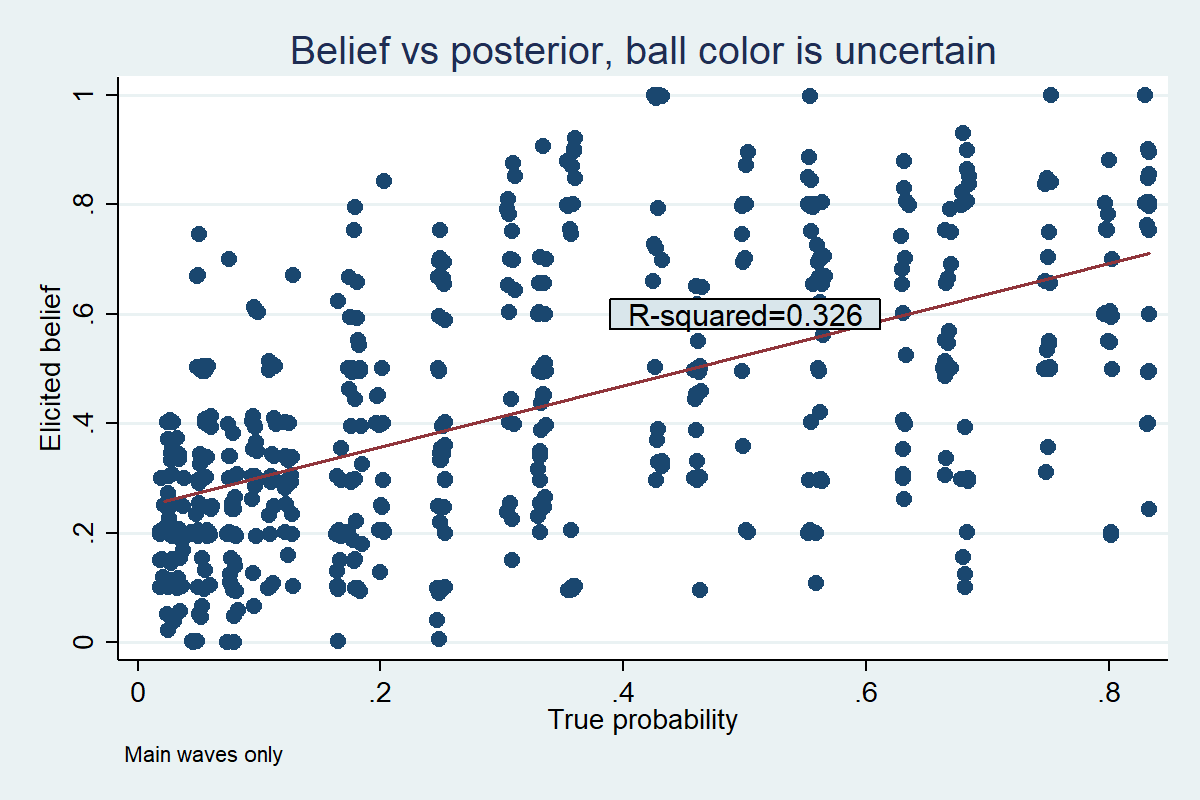
\includegraphics[width=0.9\textwidth]{Graphs/updating_s4.png}
\end{figure}
\end{center}
\end{column}
\end{columns}
\end{frame}


\begin{frame}
\frametitle{BE Big Picture}
\begin{itemize}
\item Overprotect in response to white signals, underprotect in response to black signals without false-positive: can be explained by risk preferences
\item Overprotect in response to white signals with FP (cannot be explained by risk preferences)!
\end{itemize}
\scriptsize
\begin{table}[H]\centering \caption{Average Belief Error by Signal Type} \begin{tabular}{ccccccc} \hline \hline
 & \textbf{False-pos.}&\textbf{False-neg.}&\textbf{Signal}&\textbf{Posterior}&\textbf{Belief error}& \textbf{P($=0$)}\\ \hline
(1)&No&No&White&0.000&0.050&0.000\\
(2)&No&Yes&White&0.100&0.122&0.000\\
(3)&Yes&No&White&0.000&0.122&0.000\\
(4)&Yes&Yes&White&0.131&0.218&0.000\\
(5)&No&No&Black&1.000&-0.163&0.000\\
(6)&No&Yes&Black&1.000&-0.279&0.000\\
(7)&Yes&No&Black&0.550&0.039&0.130\\
(8)&Yes&Yes&Black&0.483&0.048&0.021\\
\hline \end{tabular} \end{table}

\end{frame}



\begin{frame}
\frametitle{Distribution of WTP Discrepancies}
\begin{figure}[h]
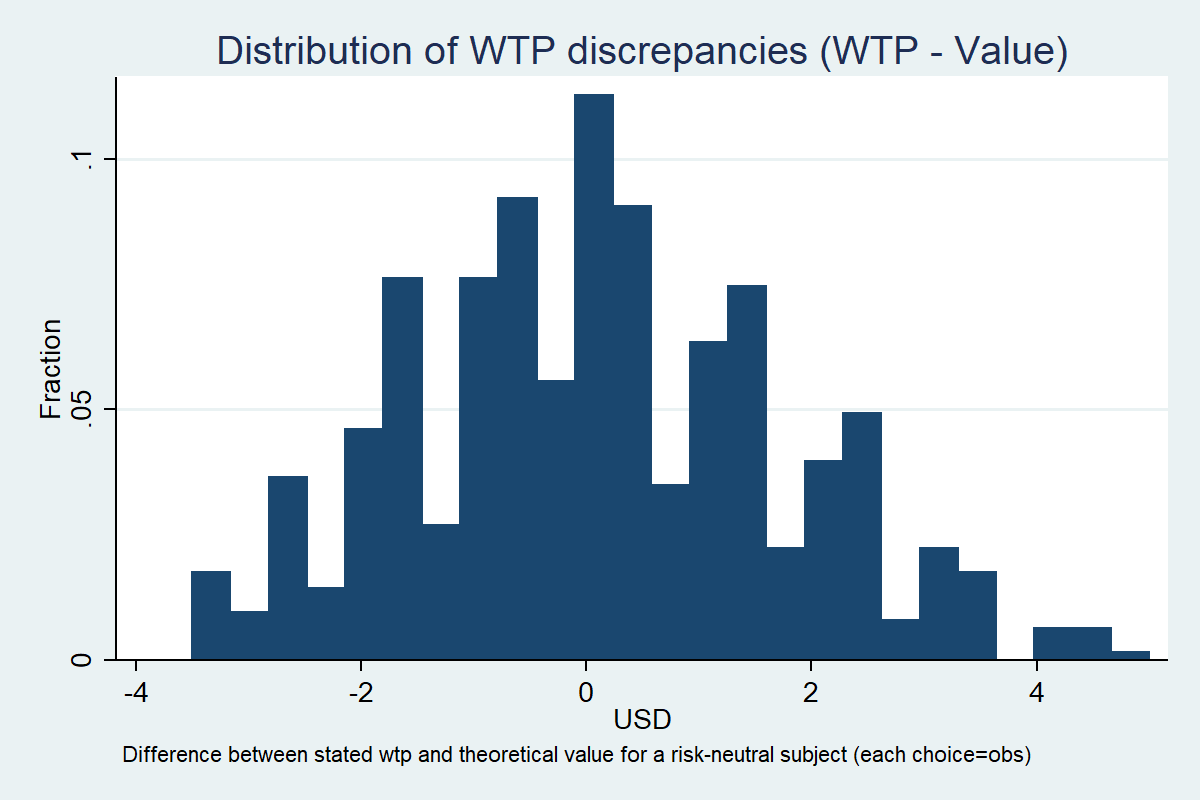
\includegraphics[scale=0.2]{Graphs/hist_WTP_discr1.png}
\end{figure}
\end{frame}





\begin{frame}
\frametitle{WTP for Signals: Big Picture}
\begin{itemize}
\item Overpaying for signals when both false-positive and false-negative events are possible
\item Small and insignificant discrepancies for other signal types
\end{itemize}
\small
\begin{table}[H]\centering \begin{tabular}{cccc} \hline \hline
\textbf{False-positive}&\textbf{False-negative}&\textbf{Mean WTP discrepancy}& \textbf{P($=0$)}\\ \hline
No&No&-0.106&0.433\\
No&Yes&0.143&0.250\\
Yes&No&0.081&0.502\\
Yes&Yes&0.492&0.000\\
\hline \end{tabular} \end{table}

\end{frame}


\begin{frame}
\frametitle{WTP for Signals}
\begin{itemize}
\item Next, we test main hypotheses of this study
\item Calculate the difference between reported WTP and theoretical WTP
\item Regress the difference on FP costs ($(1-p)P(s=1|\omega=0)c$) and FN costs ($pP(s=0|\omega=1)L$)
\item Coefficients should be zero if the theoretical model is correct
\end{itemize}
\end{frame}



\begin{frame}
\frametitle{WTP for Signals: Determinants}
\scriptsize
{
\def\sym#1{\ifmmode^{#1}\else\(^{#1}\)\fi}
\begin{tabular}{l*{5}{c}}
\hline\hline
                &\multicolumn{1}{c}{(1)}&\multicolumn{1}{c}{(2)}&\multicolumn{1}{c}{(3)}&\multicolumn{1}{c}{(4)}&\multicolumn{1}{c}{(5)}\\
                &\multicolumn{1}{c}{}&\multicolumn{1}{c}{FE}&\multicolumn{1}{c}{FE}&\multicolumn{1}{c}{FE}&\multicolumn{1}{c}{FE}\\
\hline
FP costs        &     .237\sym{*}  &     .231\sym{*}  &     .204         &     .448\sym{***}&     .412\sym{***}\\
FN costs        &     .353\sym{***}&     .319\sym{***}&     .232         &     .337\sym{***}&    -.635\sym{***}\\
Risk-loving $\times$ FP costs&                  &                  &     .165         &                  &                  \\
Risk-averse $\times$ FP costs&                  &                  &   -.0197         &                  &                  \\
No risk av. measure $\times$ FP costs&                  &                  &    .0244         &                  &                  \\
Risk-loving $\times$ FN costs&                  &                  &     .177         &                  &                  \\
Risk-averse $\times$ FN costs&                  &                  &    .0608         &                  &                  \\
No risk av. measure $\times$ FN costs&                  &                  &     .114         &                  &                  \\
Inaccurate beliefs $\times$ FP costs&                  &                  &                  &    -.197         &                  \\
Inaccurate beliefs $\times$ FN costs&                  &                  &                  &     .309         &                  \\
plevel=200 $\times$ FP costs&                  &                  &                  &                  &     .162         \\
plevel=300 $\times$ FP costs&                  &                  &                  &                  &    -.417\sym{***}\\
plevel=500 $\times$ FP costs&                  &                  &                  &                  &    -.755\sym{*}  \\
plevel=200 $\times$ FN costs&                  &                  &                  &                  &     .828\sym{***}\\
plevel=300 $\times$ FN costs&                  &                  &                  &                  &     .886\sym{***}\\
plevel=500 $\times$ FN costs&                  &                  &                  &                  &     1.02\sym{***}\\
Constant        &    -.207         &    -.182\sym{**} &    -.184\sym{**} &    -.409\sym{***}&     .575\sym{***}\\
Risk pref dummies &       No         &       No         &      Yes         &       No         &       No         \\
Prior dummies   &       No         &       No         &       No         &       No         &      Yes         \\
Belief accuracy &       No         &       No         &       No         &      Yes         &       No         \\
\hline
Observations    &      624         &      624         &      624         &      624         &      624         \\
Adjusted \(R^{2}\)&     0.05         &     0.38         &     0.37         &     0.38         &     0.58         \\
\hline\hline
\multicolumn{6}{l}{\footnotesize \sym{*} \(p<0.10\), \sym{**} \(p<0.05\), \sym{***} \(p<0.01\)}\\
\end{tabular}
}

%\begin{figure}
%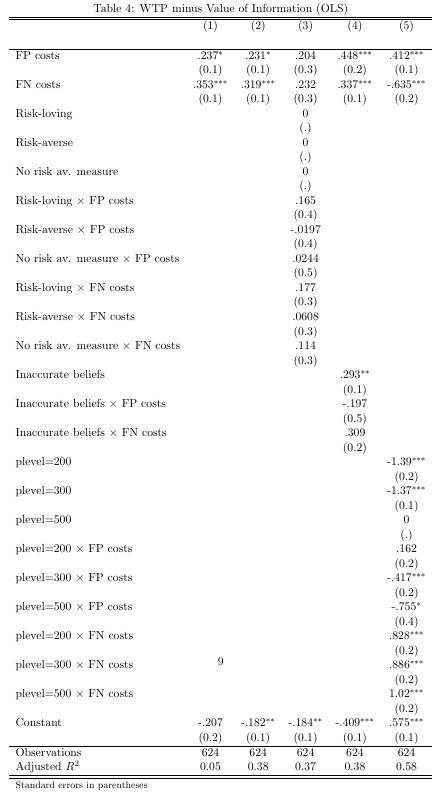
\includegraphics[width=0.9\textwidth]{WTP_determ.png}
%\end{figure}
\end{frame}



\begin{frame}
\frametitle{WTP Anomalies}
\begin{itemize}
\item No evidence of relative underweighting of FP or FN signals on average ($\beta_{FP}=\beta_{FN}$)
\item Our results exhibit the following anomaly:
\begin{enumerate}
\item Excess sensitivity to false-negative costs for low priors; lack of sensitivity for high priors
\item Underresponse to false-positive costs for low priors; excess sensitivity for high priors
\end{enumerate}
\item Next, we explore potential explanations for the anomaly
\end{itemize}
\end{frame}



\begin{frame}
\frametitle{Anomaly: Excess Sensitivity to FP/FN Costs Varies by Priors}
\begin{itemize}
\item Anomaly: we find relative overweighting of FN costs for low priors; overweighting of FP costs for high priors
\item The pattern is monotonic by priors
\end{itemize}
\footnotesize
\begin{table}[htbp]\centering
\def\sym#1{\ifmmode^{#1}\else\(^{#1}\)\fi}
\caption{WTP - Value of Information, by prior}
\begin{tabular}{l*{4}{c}}
\hline\hline
                &\multicolumn{1}{c}{(1)}&\multicolumn{1}{c}{(2)}&\multicolumn{1}{c}{(3)}&\multicolumn{1}{c}{(4)}\\
                &\multicolumn{1}{c}{0.1}&\multicolumn{1}{c}{0.2}&\multicolumn{1}{c}{0.3}&\multicolumn{1}{c}{0.5}\\
\hline
FP costs        &     .437\sym{***}&     .576\sym{***}&   -.0356         &    -.346         \\
                &    (0.1)         &    (0.2)         &    (0.2)         &    (0.3)         \\
FN costs        &    -.645\sym{***}&     .196         &     .254\sym{***}&     .379\sym{***}\\
                &    (0.2)         &    (0.1)         &    (0.1)         &    (0.1)         \\
Constant        &     .467\sym{***}&    -.713\sym{***}&    -.877\sym{***}&     .677\sym{***}\\
                &    (0.1)         &    (0.1)         &    (0.1)         &    (0.2)         \\
\hline
Observations    &      159         &      153         &      159         &      153         \\
Adjusted \(R^{2}\)&     0.63         &     0.49         &     0.40         &     0.48         \\
\hline\hline
\multicolumn{5}{l}{\footnotesize Standard errors in parentheses}\\
\multicolumn{5}{l}{\footnotesize Subject fixed effects are included.}\\
\multicolumn{5}{l}{\footnotesize \sym{*} \(p<0.10\), \sym{**} \(p<0.05\), \sym{***} \(p<0.01\)}\\
\end{tabular}
\end{table}

\end{frame}



\begin{frame}
\frametitle{Anomaly Reframed}
\begin{itemize}
\item Note that the apparent heterogeneity comes from contrasting with the theoretical value!
\item Excess sensitivity varies only because the benchmark theoretical sensitivity varies
\item The sensitivity of WTP to FP/FN rates shows little variation by prior
\end{itemize}
\scriptsize
\begin{center}
{
\def\sym#1{\ifmmode^{#1}\else\(^{#1}\)\fi}
\begin{tabular}{l*{4}{c}}
\hline\hline
                &\multicolumn{1}{c}{(1)}&\multicolumn{1}{c}{(2)}&\multicolumn{1}{c}{(3)}&\multicolumn{1}{c}{(4)}\\
                &\multicolumn{1}{c}{0.1}&\multicolumn{1}{c}{0.2}&\multicolumn{1}{c}{0.3}&\multicolumn{1}{c}{0.5}\\
\hline
FP rate         &    -2.91\sym{***}&    -2.08\sym{**} &    -4.46\sym{***}&    -3.25\sym{**} \\
                &    (1.1)         &    (1.0)         &    (1.0)         &    (1.3)         \\
FN rate         &    -2.48\sym{**} &    -2.73\sym{***}&     -3.7\sym{***}&    -3.65\sym{***}\\
                &    (1.1)         &    (1.0)         &    (1.0)         &    (1.3)         \\
\hline
Observations    &      159         &      153         &      159         &      153         \\
Adjusted \(R^{2}\)&                  &                  &                  &                  \\
\hline\hline
\multicolumn{5}{l}{\footnotesize Standard errors in parentheses}\\
\multicolumn{5}{l}{\footnotesize Tobit regression of WTP, constant omitted}\\
\multicolumn{5}{l}{\footnotesize \sym{*} \(p<0.10\), \sym{**} \(p<0.05\), \sym{***} \(p<0.01\)}\\
\end{tabular}
}

\end{center}
\end{frame}


\begin{frame}
\frametitle{Potential Explanations}
\begin{enumerate}
\item Risk preferences
\item Information preferences: paying for non-instrumental information
\item Biased beliefs:
\begin{itemize}
\item Poor differentiation between false-positive and false-negative rates (all the dishonest gremlins are equally bad)
\item Neglecting to account for priors when evaluating the frequency of FP and FN events
\end{itemize}
\end{enumerate}
\end{frame}


\begin{frame}
\frametitle{Risk Preferences Explanation}
\begin{itemize}
\item Can risk preferences within the EU framework lead to overweigting of FN costs and underweighting for FP costs for low priors and vice versa?
\item This effect is possible in theory for FN costs if subjects are risk-averse and have positive prudency. The theory gives no answer for FP costs.
\item Previous results indicate that risk aversion elicited in BP have little explanatory power for FP/FN sensitivity, but there are power issues
\item We can test it more rigorously and see if controlling for risk preferences makes the prior-FP(FN) interactions small and insignificant
\item We find that risk preferences do not explain the pattern for FN costs, but partially explain the variation for FP costs
\end{itemize}
\end{frame}


\begin{frame}
\frametitle{Risk Preferences Testing}
\scriptsize
{
\def\sym#1{\ifmmode^{#1}\else\(^{#1}\)\fi}
\begin{tabular}{l*{5}{c}}
\hline\hline
                &\multicolumn{1}{c}{(1)}&\multicolumn{1}{c}{(2)}&\multicolumn{1}{c}{(3)}&\multicolumn{1}{c}{(4)}&\multicolumn{1}{c}{(5)}\\
                &\multicolumn{1}{c}{}&\multicolumn{1}{c}{}&\multicolumn{1}{c}{}&\multicolumn{1}{c}{FE}&\multicolumn{1}{c}{FE}\\
\hline
p$>$0.2         &   -.0942         &     -.11         &   -.0409         &    -.127         &   -.0578         \\
FN costs        &    -.229         &    -.442         &    -.327         &    -.385         &     -.36         \\
p$>$0.2 $\times$ FN costs&     .716\sym{***}&     .977\sym{***}&     .889\sym{***}&     .949\sym{***}&     .914\sym{***}\\
FP costs        &     .558\sym{***}&      .69\sym{***}&      .78\sym{***}&     .652\sym{***}&     .672\sym{***}\\
p$>$0.2 $\times$ FP costs&    -.933\sym{***}&    -.879\sym{**} &    -.899\sym{**} &    -.863\sym{**} &     -.91\sym{**} \\
Risk-loving $\times$ p$>$0.2 $\times$ FN costs&                  &     .037         &    -.383         &   -.0593         &    -.276         \\
Risk-averse $\times$ p$>$0.2 $\times$ FN costs&                  &    -.245         &    -.279         &    -.372\sym{*}  &    -.198         \\
Inconsistent $\times$ p$>$0.2 $\times$ FN costs&                  &   -.0735         &    -.181         &    -.066         &    -.297         \\
Risk-loving $\times$ p$>$0.2 $\times$ FP costs&                  &    -.287         &    .0971         &     .179         &     .259         \\
Risk-averse $\times$ p$>$0.2 $\times$ FP costs&                  &    -.323         &   .00169         &     -.52         &    .0291         \\
Inconsistent $\times$ p$>$0.2 $\times$ FP costs&                  &     .108         &     -.21         &     -.48         &    -.372         \\
Full risk pref interactions&       No         &       No         &      Yes         &       No         &      Yes         \\
\hline
Observations    &      624         &      624         &      624         &      624         &      624         \\
Adjusted \(R^{2}\)&     0.08         &     0.07         &     0.07         &     0.42         &     0.42         \\
\hline\hline
\multicolumn{6}{l}{\footnotesize \sym{*} \(p<0.05\), \sym{**} \(p<0.01\), \sym{***} \(p<0.001\)}\\
\end{tabular}
}

\end{frame}




\begin{frame}
\frametitle{Paying for non-instrumental information}
\begin{itemize}
\item Humans often put positive value on information not changing their decisions (citations)
\item Signals with zero theoretical value can have positive elicited WTP
\item We see subjects paying positive amounts for signals with zero theoretical value as well as paying for signals not affecting their decisions in IP task, but it is not clear if those are reasoning mistakes or genuine preferences
\item Explaining the pattern would require non-instrumental part of value to have positive sensitivity to FP/FN rates for some priors and negative for others
\item A priori there is no reason for the non-instrumental value to \textbf{decrease} with either FP or FN costs
\end{itemize}
\end{frame}


\begin{frame}
\frametitle{Are Beliefs Biased?}
\begin{itemize}
\item We are left with biased beliefs as the anomaly explanation
\item Do choices in other tasks indicate biased beliefs?
\item Choices in BE task show obvious biases:
\begin{itemize}
\item Both the base-rate neglect and the signal underweighting
\item FN rates cause beliefs compression (lower difference in beliefs when getting black or white signals)
\end{itemize}
\item In the IP task both FP and FN rates increase protection conditional on posterior when the signal is white but have an opposite effect when the signal is black $\implies$ makes signal less valuable
\end{itemize}
\end{frame}


\begin{frame}
\frametitle{Base-rate Neglect Refresher}
\begin{itemize}
\item A standard Bayesian agent does:
$$P(B|S)={P(S|B)P(B)\over P(S|W)P(W)+P(S|B)P(B)}$$
\item More generally, consider an agent updating as a quasi-Bayesian:
$$\mu(B|S)={P(S|B)^{\alpha}P(B){\beta}\over P(S|W)^{\alpha} P(W)^{\beta}+P(S|B)^{\alpha}P(B)^{\beta}} $$
\item One can estimate it as:
$$\log\left({\mu(B|S) \over 1-\mu(B|S)}\right)=\alpha \log\left({P(S|B) \over P(S|W)}\right)+\beta \log \left({P(B)\over P(W)}\right)$$
\item Base-rate neglect is when $0<\beta<1$ and $0<\alpha<1$ is the signal underweighting
\item We find both
\end{itemize}
\end{frame}


\begin{frame}
\frametitle{Base-rate neglect and signal underweighting in BE data}
\footnotesize
\begin{table}[htbp]\centering
\def\sym#1{\ifmmode^{#1}\else\(^{#1}\)\fi}
\caption{Belief Elicitation: Decomposition}
\begin{tabular}{l*{3}{c}}
\hline\hline
                &\multicolumn{1}{c}{(1)}&\multicolumn{1}{c}{(2)}&\multicolumn{1}{c}{(3)}\\
                &\multicolumn{1}{c}{OLS}&\multicolumn{1}{c}{FE}&\multicolumn{1}{c}{Smart, FE}\\
\hline
lt\_prior        &     .178         &     .205\sym{**} &     .231\sym{**} \\
                &    (1.4)         &    (2.5)         &    (2.2)         \\
signalB         &   -.0835         &     .735\sym{**} &     .988\sym{**} \\
                &   (-0.2)         &    (2.5)         &    (2.5)         \\
signalW         &     .818\sym{***}&        0         &        0         \\
                &    (2.8)         &      (.)         &      (.)         \\
Constant        &     .332         &    -.471\sym{**} &    -.577\sym{**} \\
                &    (0.9)         &   (-2.7)         &   (-2.6)         \\
\hline
Observations    &       68         &       68         &       52         \\
Adjusted \(R^{2}\)&     0.16         &     0.20         &     0.25         \\
\hline\hline
\multicolumn{4}{l}{\footnotesize \textit{t} statistics in parentheses}\\
\multicolumn{4}{l}{\footnotesize \sym{*} \(p<0.10\), \sym{**} \(p<0.05\), \sym{***} \(p<0.01\)}\\
\end{tabular}
\end{table}

\end{frame}



\begin{frame}
\frametitle{Belief Biases by FP/FN rates}
\begin{itemize}
\item FN rates induce positive belief bias for white signals and negative bias for black signals $\implies$ lowers the difference between beliefs when black/white balls
\item FP rates induce positive bias both for white signals and for black signals $\implies$ the difference decreases for priors$\leq$0.2 and increases otherwise
\end{itemize}
\scriptsize
\begin{table}[htbp]\centering
\def\sym#1{\ifmmode^{#1}\else\(^{#1}\)\fi}
\caption{Belief Elicitation: When Mistakes Happen}
\begin{tabular}{l*{3}{c}}
\hline\hline
                &\multicolumn{1}{c}{(1)}&\multicolumn{1}{c}{(2)}&\multicolumn{1}{c}{(3)}\\
                &\multicolumn{1}{c}{All}&\multicolumn{1}{c}{S=White}&\multicolumn{1}{c}{S=Black}\\
\hline
FP rate         &    0.600\sym{***}&    0.292\sym{***}&    0.908\sym{***}\\
                &  (0.057)         &  (0.063)         &  (0.102)         \\
FN rate         &    0.011         &    0.273\sym{***}&   -0.251\sym{***}\\
                &  (0.053)         &  (0.061)         &  (0.084)         \\
A92             &   -0.018\sym{*}  &   -0.145\sym{***}&    0.108\sym{***}\\
                &  (0.009)         &  (0.010)         &  (0.016)         \\
B113            &   -0.088\sym{***}&   -0.372\sym{***}&    0.196\sym{***}\\
                &  (0.009)         &  (0.010)         &  (0.016)         \\
B139            &    0.140\sym{***}&   -0.190\sym{***}&    0.470\sym{***}\\
                &  (0.000)         &  (0.000)         &  (0.000)         \\
B61             &   -0.170\sym{***}&   -0.177\sym{***}&   -0.163\sym{***}\\
                &  (0.000)         &  (0.000)         &  (0.000)         \\
B87             &    0.084\sym{***}&   -0.305\sym{***}&    0.473\sym{***}\\
                &  (0.001)         &  (0.001)         &  (0.002)         \\
C108            &    0.104\sym{***}&   -0.299\sym{***}&    0.506\sym{***}\\
                &  (0.001)         &  (0.001)         &  (0.002)         \\
C134            &    0.006         &   -0.205\sym{***}&    0.217\sym{***}\\
                &  (0.009)         &  (0.010)         &  (0.016)         \\
C56             &    0.005         &   -0.326\sym{***}&    0.337\sym{***}\\
                &  (0.009)         &  (0.010)         &  (0.016)         \\
C82             &    0.056\sym{***}&   -0.248\sym{***}&    0.360\sym{***}\\
                &  (0.000)         &  (0.000)         &  (0.000)         \\
D103            &    0.123\sym{***}&   -0.207\sym{***}&    0.453\sym{***}\\
                &  (0.000)         &  (0.000)         &  (0.000)         \\
D129            &    0.086\sym{***}&   -0.326\sym{***}&    0.498\sym{***}\\
                &  (0.001)         &  (0.001)         &  (0.002)         \\
D51             &    0.070\sym{***}&   -0.241\sym{***}&    0.381\sym{***}\\
                &  (0.001)         &  (0.001)         &  (0.002)         \\
D77             &    0.024\sym{**} &   -0.289\sym{***}&    0.337\sym{***}\\
                &  (0.009)         &  (0.010)         &  (0.016)         \\
E124            &    0.084\sym{***}&   -0.350\sym{***}&    0.518\sym{***}\\
                &  (0.000)         &  (0.000)         &  (0.000)         \\
E150            &    0.125\sym{***}&   -0.312\sym{***}&    0.561\sym{***}\\
                &  (0.001)         &  (0.001)         &  (0.002)         \\
E46             &    0.052\sym{***}&   -0.340\sym{***}&    0.443\sym{***}\\
                &  (0.000)         &  (0.000)         &  (0.000)         \\
E72             &    0.071\sym{***}&   -0.265\sym{***}&    0.406\sym{***}\\
                &  (0.001)         &  (0.001)         &  (0.002)         \\
E98             &    0.142\sym{***}&   -0.116\sym{***}&    0.400\sym{***}\\
                &  (0.009)         &  (0.010)         &  (0.016)         \\
F119            &    0.003         &   -0.314\sym{***}&    0.319\sym{***}\\
                &  (0.009)         &  (0.010)         &  (0.016)         \\
F41             &    0.080\sym{***}&   -0.307\sym{***}&    0.467\sym{***}\\
                &  (0.009)         &  (0.010)         &  (0.016)         \\
F67             &    0.123\sym{***}&   -0.334\sym{***}&    0.580\sym{***}\\
                &  (0.000)         &  (0.000)         &  (0.000)         \\
F93             &    0.093\sym{***}&   -0.305\sym{***}&    0.490\sym{***}\\
                &  (0.001)         &  (0.001)         &  (0.002)         \\
G114            &    0.122\sym{***}&   -0.284\sym{***}&    0.528\sym{***}\\
                &  (0.001)         &  (0.001)         &  (0.002)         \\
G140            &   -0.023\sym{**} &   -0.065\sym{***}&    0.018         \\
                &  (0.009)         &  (0.010)         &  (0.016)         \\
G62             &   -0.002         &   -0.425\sym{***}&    0.420\sym{***}\\
                &  (0.009)         &  (0.010)         &  (0.016)         \\
G88             &    0.039\sym{***}&   -0.315\sym{***}&    0.393\sym{***}\\
                &  (0.000)         &  (0.000)         &  (0.000)         \\
H109            &    0.122\sym{***}&   -0.287\sym{***}&    0.532\sym{***}\\
                &  (0.000)         &  (0.000)         &  (0.000)         \\
H135            &    0.070\sym{***}&   -0.341\sym{***}&    0.481\sym{***}\\
                &  (0.001)         &  (0.001)         &  (0.002)         \\
H57             &   -0.022\sym{***}&   -0.301\sym{***}&    0.256\sym{***}\\
                &  (0.001)         &  (0.001)         &  (0.002)         \\
H83             &    0.082\sym{***}&   -0.280\sym{***}&    0.444\sym{***}\\
                &  (0.009)         &  (0.010)         &  (0.016)         \\
I104            &   -0.003         &   -0.193\sym{***}&    0.187\sym{***}\\
                &  (0.009)         &  (0.010)         &  (0.016)         \\
I130            &    0.090\sym{***}&   -0.247\sym{***}&    0.427\sym{***}\\
                &  (0.000)         &  (0.000)         &  (0.000)         \\
I52             &    0.010\sym{***}&   -0.215\sym{***}&    0.235\sym{***}\\
                &  (0.000)         &  (0.000)         &  (0.000)         \\
I78             &    0.127\sym{***}&   -0.277\sym{***}&    0.531\sym{***}\\
                &  (0.001)         &  (0.001)         &  (0.002)         \\
J125            &    0.037\sym{***}&   -0.047\sym{***}&    0.121\sym{***}\\
                &  (0.009)         &  (0.010)         &  (0.016)         \\
J151            &   -0.043\sym{***}&   -0.157\sym{***}&    0.070\sym{***}\\
                &  (0.000)         &  (0.000)         &  (0.000)         \\
J47             &    0.073\sym{***}&   -0.264\sym{***}&    0.409\sym{***}\\
                &  (0.009)         &  (0.010)         &  (0.016)         \\
J73             &    0.162\sym{***}&   -0.212\sym{***}&    0.537\sym{***}\\
                &  (0.000)         &  (0.000)         &  (0.000)         \\
J99             &    0.041\sym{***}&   -0.235\sym{***}&    0.316\sym{***}\\
                &  (0.001)         &  (0.001)         &  (0.002)         \\
K120            &    0.127\sym{***}&   -0.277\sym{***}&    0.531\sym{***}\\
                &  (0.001)         &  (0.001)         &  (0.002)         \\
K42             &    0.004\sym{***}&   -0.324\sym{***}&    0.331\sym{***}\\
                &  (0.001)         &  (0.001)         &  (0.002)         \\
K68             &    0.035\sym{***}&   -0.213\sym{***}&    0.283\sym{***}\\
                &  (0.009)         &  (0.010)         &  (0.016)         \\
K94             &    0.056\sym{***}&   -0.298\sym{***}&    0.410\sym{***}\\
                &  (0.000)         &  (0.000)         &  (0.000)         \\
L115            &    0.081\sym{***}&   -0.152\sym{***}&    0.313\sym{***}\\
                &  (0.000)         &  (0.000)         &  (0.000)         \\
L141            &   -0.056\sym{***}&   -0.201\sym{***}&    0.090\sym{***}\\
                &  (0.001)         &  (0.001)         &  (0.002)         \\
L63             &    0.056\sym{***}&   -0.320\sym{***}&    0.431\sym{***}\\
                &  (0.001)         &  (0.001)         &  (0.002)         \\
L89             &    0.089\sym{***}&   -0.135\sym{***}&    0.314\sym{***}\\
                &  (0.009)         &  (0.010)         &  (0.016)         \\
M110            &    0.008         &   -0.033\sym{***}&    0.048\sym{***}\\
                &  (0.009)         &  (0.010)         &  (0.016)         \\
M136            &   -0.057\sym{***}&   -0.232\sym{***}&    0.118\sym{***}\\
                &  (0.000)         &  (0.000)         &  (0.000)         \\
M58             &   -0.094\sym{***}&   -0.382\sym{***}&    0.193\sym{***}\\
                &  (0.000)         &  (0.000)         &  (0.000)         \\
M84             &   -0.196\sym{***}&   -0.190\sym{***}&   -0.202\sym{***}\\
                &  (0.001)         &  (0.001)         &  (0.002)         \\
N105            &   -0.048\sym{***}&   -0.328\sym{***}&    0.231\sym{***}\\
                &  (0.001)         &  (0.001)         &  (0.002)         \\
N131            &   -0.019\sym{**} &   -0.409\sym{***}&    0.371\sym{***}\\
                &  (0.009)         &  (0.010)         &  (0.016)         \\
N53             &    0.039\sym{***}&   -0.414\sym{***}&    0.492\sym{***}\\
                &  (0.009)         &  (0.010)         &  (0.016)         \\
N79             &    0.078\sym{***}&   -0.375\sym{***}&    0.532\sym{***}\\
                &  (0.000)         &  (0.000)         &  (0.000)         \\
O100            &   -0.111\sym{***}&   -0.348\sym{***}&    0.127\sym{***}\\
                &  (0.000)         &  (0.000)         &  (0.000)         \\
O126            &    0.066\sym{***}&   -0.347\sym{***}&    0.478\sym{***}\\
                &  (0.001)         &  (0.001)         &  (0.002)         \\
O48             &   -0.206\sym{***}&   -0.200\sym{***}&   -0.212\sym{***}\\
                &  (0.001)         &  (0.001)         &  (0.002)         \\
O74             &    0.059\sym{***}&   -0.313\sym{***}&    0.430\sym{***}\\
                &  (0.009)         &  (0.010)         &  (0.016)         \\
P121            &    0.115\sym{***}&   -0.250\sym{***}&    0.480\sym{***}\\
                &  (0.000)         &  (0.000)         &  (0.000)         \\
P43             &    0.108\sym{***}&   -0.207\sym{***}&    0.423\sym{***}\\
                &  (0.000)         &  (0.000)         &  (0.000)         \\
P69             &   -0.272\sym{***}&   -0.251\sym{***}&   -0.294\sym{***}\\
                &  (0.001)         &  (0.001)         &  (0.002)         \\
P95             &    0.073\sym{***}&   -0.297\sym{***}&    0.442\sym{***}\\
                &  (0.009)         &  (0.010)         &  (0.016)         \\
Q116            &   -0.004         &   -0.423\sym{***}&    0.415\sym{***}\\
                &  (0.009)         &  (0.010)         &  (0.016)         \\
Q142            &    0.056\sym{***}&   -0.248\sym{***}&    0.360\sym{***}\\
                &  (0.000)         &  (0.000)         &  (0.000)         \\
Q64             &    0.102\sym{***}&   -0.248\sym{***}&    0.452\sym{***}\\
                &  (0.000)         &  (0.000)         &  (0.000)         \\
Q90             &   -0.181\sym{***}&   -0.259\sym{***}&   -0.104\sym{***}\\
                &  (0.001)         &  (0.001)         &  (0.002)         \\
R111            &   -0.089\sym{***}&   -0.068\sym{***}&   -0.110\sym{***}\\
                &  (0.001)         &  (0.001)         &  (0.002)         \\
R137            &   -0.190\sym{***}&   -0.294\sym{***}&   -0.086\sym{***}\\
                &  (0.009)         &  (0.010)         &  (0.016)         \\
R59             &    0.080\sym{***}&   -0.322\sym{***}&    0.482\sym{***}\\
                &  (0.009)         &  (0.010)         &  (0.016)         \\
R85             &    0.120\sym{***}&   -0.269\sym{***}&    0.508\sym{***}\\
                &  (0.000)         &  (0.000)         &  (0.000)         \\
S106            &   -0.344\sym{***}&   -0.348\sym{***}&   -0.340\sym{***}\\
                &  (0.000)         &  (0.000)         &  (0.000)         \\
S132            &    0.121\sym{***}&   -0.319\sym{***}&    0.561\sym{***}\\
                &  (0.001)         &  (0.001)         &  (0.002)         \\
S54             &    0.119\sym{***}&   -0.312\sym{***}&    0.550\sym{***}\\
                &  (0.001)         &  (0.001)         &  (0.002)         \\
S80             &    0.029\sym{***}&   -0.283\sym{***}&    0.342\sym{***}\\
                &  (0.009)         &  (0.010)         &  (0.016)         \\
T101            &   -0.025\sym{***}&   -0.349\sym{***}&    0.299\sym{***}\\
                &  (0.009)         &  (0.010)         &  (0.016)         \\
T127            &    0.102\sym{***}&   -0.324\sym{***}&    0.528\sym{***}\\
                &  (0.000)         &  (0.000)         &  (0.000)         \\
T49             &   -0.127\sym{***}&   -0.224\sym{***}&   -0.030\sym{***}\\
                &  (0.000)         &  (0.000)         &  (0.000)         \\
T75             &    0.048\sym{***}&   -0.343\sym{***}&    0.440\sym{***}\\
                &  (0.001)         &  (0.001)         &  (0.002)         \\
U122            &    0.022\sym{**} &   -0.375\sym{***}&    0.418\sym{***}\\
                &  (0.009)         &  (0.010)         &  (0.016)         \\
U44             &    0.021\sym{**} &   -0.408\sym{***}&    0.450\sym{***}\\
                &  (0.009)         &  (0.010)         &  (0.016)         \\
U70             &    0.089\sym{***}&   -0.290\sym{***}&    0.468\sym{***}\\
                &  (0.000)         &  (0.000)         &  (0.000)         \\
U96             &   -0.035\sym{***}&   -0.195\sym{***}&    0.125\sym{***}\\
                &  (0.001)         &  (0.001)         &  (0.002)         \\
V117            &    0.072\sym{***}&   -0.338\sym{***}&    0.481\sym{***}\\
                &  (0.001)         &  (0.001)         &  (0.002)         \\
V65             &    0.137\sym{***}&   -0.110\sym{***}&    0.384\sym{***}\\
                &  (0.009)         &  (0.010)         &  (0.016)         \\
V91             &    0.107\sym{***}&   -0.249\sym{***}&    0.462\sym{***}\\
                &  (0.000)         &  (0.000)         &  (0.000)         \\
W112            &    0.101\sym{***}&   -0.225\sym{***}&    0.427\sym{***}\\
                &  (0.000)         &  (0.000)         &  (0.000)         \\
W138            &   -0.088\sym{***}&   -0.232\sym{***}&    0.056\sym{***}\\
                &  (0.001)         &  (0.001)         &  (0.002)         \\
W60             &   -0.038\sym{***}&   -0.257\sym{***}&    0.181\sym{***}\\
                &  (0.001)         &  (0.001)         &  (0.002)         \\
W86             &    0.008         &   -0.351\sym{***}&    0.367\sym{***}\\
                &  (0.009)         &  (0.010)         &  (0.016)         \\
X107            &   -0.097\sym{***}&   -0.380\sym{***}&    0.187\sym{***}\\
                &  (0.009)         &  (0.010)         &  (0.016)         \\
X133            &   -0.227\sym{***}&   -0.232\sym{***}&   -0.222\sym{***}\\
                &  (0.000)         &  (0.000)         &  (0.000)         \\
X55             &   -0.177\sym{***}&   -0.190\sym{***}&   -0.163\sym{***}\\
                &  (0.000)         &  (0.000)         &  (0.000)         \\
X81             &   -0.089\sym{***}&   -0.218\sym{***}&    0.040\sym{***}\\
                &  (0.001)         &  (0.001)         &  (0.002)         \\
Y102            &    0.105\sym{***}&   -0.302\sym{***}&    0.511\sym{***}\\
                &  (0.001)         &  (0.001)         &  (0.002)         \\
Y128            &   -0.020\sym{**} &   -0.068\sym{***}&    0.028\sym{*}  \\
                &  (0.009)         &  (0.010)         &  (0.016)         \\
Y50             &   -0.055\sym{***}&   -0.368\sym{***}&    0.258\sym{***}\\
                &  (0.009)         &  (0.010)         &  (0.016)         \\
Y76             &    0.093\sym{***}&   -0.248\sym{***}&    0.435\sym{***}\\
                &  (0.000)         &  (0.000)         &  (0.000)         \\
Z123            &   -0.043\sym{***}&   -0.351\sym{***}&    0.265\sym{***}\\
                &  (0.001)         &  (0.001)         &  (0.002)         \\
Z149            &    0.141\sym{***}&    0.118\sym{***}&    0.164\sym{***}\\
                &  (0.009)         &  (0.010)         &  (0.016)         \\
Z45             &   -0.157\sym{***}&   -0.276\sym{***}&   -0.039\sym{***}\\
                &  (0.001)         &  (0.001)         &  (0.002)         \\
Z71             &    0.031\sym{***}&   -0.399\sym{***}&    0.461\sym{***}\\
                &  (0.009)         &  (0.010)         &  (0.016)         \\
Z97             &    0.066\sym{***}&    0.035\sym{***}&    0.097\sym{***}\\
                &  (0.000)         &  (0.000)         &  (0.000)         \\
Constant        &   -0.078\sym{***}&    0.314\sym{***}&   -0.470\sym{***}\\
                &  (0.007)         &  (0.009)         &  (0.013)         \\
\hline
Observations    &     1248         &      624         &      624         \\
Adjusted \(R^{2}\)&    0.146         &    0.415         &    0.521         \\
\hline\hline
\multicolumn{4}{l}{\footnotesize Standard errors in parentheses}\\
\multicolumn{4}{l}{\footnotesize Dep. variable: reported belief - posterior probability}\\
\multicolumn{4}{l}{\footnotesize \sym{*} \(p<0.10\), \sym{**} \(p<0.05\), \sym{***} \(p<0.01\)}\\
\end{tabular}
\end{table}

\end{frame}



\begin{frame}
\frametitle{Protection Biases in Informed Protection}
\begin{itemize}
\item Estimate sensitivity to FP and FN rates by signal type and with flexible controls for posteriors
\item Any excess sensitivity with flexible controls for posteriors $\implies$ anomaly with respect to EU
\item Find following anomalies:
\begin{itemize}
\item FP rates increase protection when the signal is white; the same is true for FN rates but not statistically significant
\item Black signals increase protection conditional on posteriors
\item Adding flexible controls for beliefs reduces these biases
\end{itemize}
\end{itemize}
\end{frame}



\begin{frame}
\frametitle{Protection Biases in Informed Protection: Results}
\scriptsize
\begin{center}
{
\def\sym#1{\ifmmode^{#1}\else\(^{#1}\)\fi}
\begin{tabular}{l*{4}{c}}
\hline\hline
                &\multicolumn{1}{c}{(1)}&\multicolumn{1}{c}{(2)}&\multicolumn{1}{c}{(3)}&\multicolumn{1}{c}{(4)}\\
                &\multicolumn{1}{c}{}&\multicolumn{1}{c}{}&\multicolumn{1}{c}{}&\multicolumn{1}{c}{}\\
\hline
FP rate x (S=White)&     .434\sym{***}&     .508\sym{***}&     .235\sym{*}  &     .293\sym{**} \\
                &    (3.2)         &    (3.4)         &    (1.8)         &    (2.0)         \\
FN rate x (S=White)&      .43\sym{*}  &     .412         &    .0513         &    .0366         \\
                &    (1.8)         &    (1.7)         &    (0.2)         &    (0.1)         \\
FP rate x (S=Black)&    -.128         &   -.0328         &    -.187         &    -.114         \\
                &   (-0.3)         &   (-0.1)         &   (-0.4)         &   (-0.2)         \\
FN rate x (S=Black)&    .0434         &    -.067         &  .000394         &   -.0827         \\
                &    (0.4)         &   (-0.4)         &    (0.0)         &   (-0.5)         \\
S=Black         &     .342\sym{*}  &     .382\sym{*}  &     .196         &     .225         \\
                &    (2.0)         &    (1.8)         &    (1.1)         &    (1.1)         \\
p$>$0.2         &    .0504\sym{**} &    .0434\sym{*}  &    .0299         &    .0251         \\
                &    (2.5)         &    (1.9)         &    (1.5)         &    (1.1)         \\
FP rate x (p$>$0.2)&                  &    -.131         &                  &    -.101         \\
                &                  &   (-0.8)         &                  &   (-0.6)         \\
FN rate x (p$>$0.2)&                  &     .221         &                  &     .165         \\
                &                  &    (1.3)         &                  &    (1.1)         \\
Subject FE      &      Yes         &      Yes         &      Yes         &      Yes         \\
Posterior       &      Yes         &      Yes         &      Yes         &      Yes         \\
Beliefs         &       No         &       No         &      Yes         &      Yes         \\
\hline
Observations    &     1248         &     1248         &     1248         &     1248         \\
Adjusted \(R^{2}\)&     0.53         &     0.53         &     0.55         &     0.55         \\
\hline\hline
\multicolumn{5}{l}{\footnotesize \textit{t} statistics in parentheses}\\
\multicolumn{5}{l}{\footnotesize \sym{*} \(p<0.10\), \sym{**} \(p<0.05\), \sym{***} \(p<0.01\)}\\
\end{tabular}
}

\end{center}
\end{frame}


\begin{frame}
\frametitle{Do Subjects Differentiate between FP and FN rates in WTP treatment?}
\begin{itemize}
\item The flatness of response to FP/FN rates with respect to priors can also be explained by subjects not distinguishing between FP and FN rates
\item Priors have opposite effects on the frequency of FP/FN events and these effects can partially cancel each other
\item Test for coefficients equality on (cost-weighted) FP/FN rates 
\item $\implies$ Cannot reject the hypothesis that the coefficients are equal
\item Reservation: mixed evidence for Informed Protection
\end{itemize}
\end{frame}


\begin{frame}
\frametitle{Differentiation of FP and FN Rates: Results}
\scriptsize
{
\def\sym#1{\ifmmode^{#1}\else\(^{#1}\)\fi}
\begin{tabular}{l*{4}{c}}
\hline\hline
                &\multicolumn{1}{c}{(1)}&\multicolumn{1}{c}{(2)}&\multicolumn{1}{c}{(3)}&\multicolumn{1}{c}{(4)}\\
                &\multicolumn{1}{c}{}&\multicolumn{1}{c}{}&\multicolumn{1}{c}{FE}&\multicolumn{1}{c}{FE}\\
\hline
FN rate         &    -2.57\sym{***}&                  &    -2.53\sym{***}&                  \\
                &    (0.4)         &                  &    (0.4)         &                  \\
FP rate         &    -2.33\sym{***}&                  &    -2.61\sym{***}&                  \\
                &    (0.5)         &                  &    (0.5)         &                  \\
plevel=200 $\times$ FN rate&                  &    -2.23\sym{***}&                  &    -2.18\sym{***}\\
                &                  &    (0.5)         &                  &    (0.5)         \\
plevel=300 $\times$ FN rate&                  &    -2.99\sym{***}&                  &    -2.97\sym{***}\\
                &                  &    (0.6)         &                  &    (0.6)         \\
plevel=500 $\times$ FN rate&                  &    -2.81\sym{***}&                  &    -2.77\sym{***}\\
                &                  &    (0.7)         &                  &    (0.7)         \\
plevel=200 $\times$ FP rate&                  &    -1.66\sym{**} &                  &    -1.89\sym{***}\\
                &                  &    (0.7)         &                  &    (0.7)         \\
plevel=300 $\times$ FP rate&                  &    -3.31\sym{***}&                  &    -3.63\sym{***}\\
                &                  &    (0.8)         &                  &    (0.8)         \\
plevel=500 $\times$ FP rate&                  &    -2.42\sym{***}&                  &    -2.66\sym{***}\\
                &                  &    (0.9)         &                  &    (0.9)         \\
\hline
P(FP rate=FN rate)&     .661         &     .862         &     .853         &      .91         \\
Adjusted \(R^{2}\)&      .16         &     .156         &     .543         &     .543         \\
Observations    &      624         &      624         &      624         &      624         \\
\hline\hline
\multicolumn{5}{l}{\footnotesize Standard errors in parentheses}\\
\multicolumn{5}{l}{\footnotesize \sym{*} \(p<0.10\), \sym{**} \(p<0.05\), \sym{***} \(p<0.01\)}\\
\end{tabular}
}

\end{frame}



\begin{frame}
\frametitle{Differentiation of FP and FN rates: Informed Protection}
\begin{itemize}
\item Evidence is mixed for the Informed Protection tasks
\item We can reject the equality hypothesis at 5\% significance for some specifications, but not for others
\item Sensitivity to FP and FN rates also varies with priors
\item It seems that subjects simplify their treatment/use heuristics when determining WTP but not when choosing protective actions as those are simpler
\item Another option: heterogeneity with respect to strategies. However, while IP choices exhibit strategy heterogeneity, IP strategies do not predict WTP choices
\end{itemize}
\end{frame}


\begin{frame}
\frametitle{Differentiation of FP and FN Rates: IP Evidence}
\scriptsize
\begin{table}[htbp]\centering
\def\sym#1{\ifmmode^{#1}\else\(^{#1}\)\fi}
\caption{Informed protection response: linear regression}
\begin{tabular}{l*{6}{c}}
\hline\hline
                &\multicolumn{1}{c}{(1)}&\multicolumn{1}{c}{(2)}&\multicolumn{1}{c}{(3)}&\multicolumn{1}{c}{(4)}&\multicolumn{1}{c}{(5)}&\multicolumn{1}{c}{(6)}\\
                &\multicolumn{1}{c}{All}&\multicolumn{1}{c}{S=White}&\multicolumn{1}{c}{S=Black}&\multicolumn{1}{c}{All}&\multicolumn{1}{c}{S=White}&\multicolumn{1}{c}{W=Black}\\
\hline
FP rate         &     .276\sym{***}&     .524\sym{***}&    .0274         &     .284\sym{***}&     .496\sym{***}&    .0725         \\
                &    (3.0)         &    (4.0)         &    (0.2)         &    (2.9)         &    (3.8)         &    (0.5)         \\
FN rate         &     .616\sym{***}&     1.23\sym{***}&   .00395         &     .596\sym{***}&     1.21\sym{***}&   -.0213         \\
                &    (7.6)         &    (9.7)         &    (0.0)         &    (7.2)         &    (8.9)         &   (-0.2)         \\
plevel=200      &     .106\sym{***}&    .0911\sym{*}  &     .121\sym{**} &     .382\sym{***}&     .693\sym{***}&    .0718\sym{***}\\
                &    (2.8)         &    (1.9)         &    (2.2)         &   (22.5)         &   (27.9)         &    (2.8)         \\
plevel=300      &     .167\sym{***}&     .164\sym{***}&      .17\sym{***}&     .167\sym{***}&     .164\sym{***}&      .17\sym{***}\\
                &    (6.7)         &    (6.2)         &    (4.0)         &    (6.4)         &    (5.7)         &    (3.6)         \\
plevel=500      &     .174\sym{***}&     .202\sym{***}&     .147\sym{***}&     .451\sym{***}&     .804\sym{***}&     .098\sym{***}\\
                &    (4.5)         &    (4.1)         &    (2.7)         &   (26.6)         &   (32.4)         &    (3.9)         \\
Constant        &     .334\sym{***}&   -.0699\sym{**} &     .738\sym{***}&     .402\sym{***}&     -.11\sym{***}&     .913\sym{***}\\
                &   (10.8)         &   (-2.2)         &   (14.4)         &   (22.5)         &   (-4.7)         &   (31.6)         \\
Subject FE      &       No         &       No         &       No         &      Yes         &      Yes         &      Yes         \\
\hline
Observations    &     1248         &      624         &      624         &     1248         &      624         &      624         \\
Adjusted \(R^{2}\)&     0.06         &     0.23         &     0.03         &     0.08         &     0.41         &     0.28         \\
\hline\hline
\multicolumn{7}{l}{\footnotesize \textit{t} statistics in parentheses}\\
\multicolumn{7}{l}{\footnotesize Errors are clustered by subject}\\
\multicolumn{7}{l}{\footnotesize \sym{*} \(p<0.10\), \sym{**} \(p<0.05\), \sym{***} \(p<0.01\)}\\
\end{tabular}
\end{table}

\end{frame}




\begin{frame}
\frametitle{Do Subjects Neglect to Account for Frequency of FP/FN events?}
\begin{itemize}
\item The anomaly is also consistent with subject neglecting prior probabilities when evaluating the effects of FP and FN rates:
\begin{itemize}
\item For the same FN rate $P(s=0|\omega=1)$, FN event is more likely when the priors are high as its probability is $pP(s=0|\omega=1)$ (the reverse is true for FP)
\item In contrast, experimental subjects reduce WTP with FP/FN rates but do it uniformly for all the priors
\item Priors still affect demand but only directly
\end{itemize}
\item This is a reasonable heuristic to evaluate the value of information: account for priors, and correct according to false-positive and false-negative rates (these variables are immediately given and do not require extra computation)
\end{itemize}
\end{frame}



\begin{frame}
\frametitle{Neglecting Frequency of FP/FN events}
\begin{itemize}
\item We can test this explanation using WTP data in two ways:
\begin{itemize}
\item Rewrite the interaction as the base rate plus interaction and test the joint significance of the interaction terms
\item Test for joint significance of the full set of flexible interactions betwen prior levels and FP/FN rates
\end{itemize}
\item The first test cannot reject the null hypothesis, but the interaction terms are jointly significant (with or without FE) at 5\%
\item The change in explanatory power is very small and coefficient magnitudes are non-sensical (smaller for 0.3 rather than for 0.5)
\end{itemize}
\end{frame}


\begin{frame}
\frametitle{Neglecting Frequency of FP/FN events}
\scriptsize
\begin{tabular}{l*{4}{c}}
\hline\hline
                &\multicolumn{1}{c}{(1)}&\multicolumn{1}{c}{(2)}&\multicolumn{1}{c}{(3)}&\multicolumn{1}{c}{(4)}\\
                &\multicolumn{1}{c}{}&\multicolumn{1}{c}{}&\multicolumn{1}{c}{}&\multicolumn{1}{c}{FE}\\
\hline
Prior\_change$\times$FP rate&    -.392&         &    -.457&         \\
                &  (0.468)&         &  (0.434)&         \\
Prior\_change$\times$FN rate&   -.0869&         &     -.08&         \\
                &  (0.089)&         &  (0.086)&         \\
plevel=200 $\times$ FP rate&         &    .0497&         &    .0668\\
                &         &  (0.197)&         &  (0.192)\\
plevel=300 $\times$ FP rate&         &    -.281&         &    -.281\\
                &         &  (0.105)&         &  (0.105)\\
plevel=500 $\times$ FP rate&         &    -.103&         &   -.0857\\
                &         &  (0.222)&         &  (0.223)\\
plevel=200 $\times$ FN rate&         & -.000453&         &  .000683\\
                &         &  (0.035)&         &  (0.032)\\
plevel=300 $\times$ FN rate&         &   -.0384&         &   -.0384\\
                &         &  (0.021)&         &  (0.021)\\
plevel=500 $\times$ FN rate&         &   -.0295&         &   -.0284\\
                &         &  (0.044)&         &  (0.040)\\
\hline
P(beta\_X=0)     &     .544&    .0286&      .53&    .0276\\
Adjusted \(R^{2}\)&     .158&     .156&     .543&     .543\\
Observations    &      624&      624&      624&      624\\
\hline\hline
\multicolumn{5}{l}{\footnotesize Standard errors in parentheses}\\
\multicolumn{5}{l}{\footnotesize Controlling for FP/FN rates, prior, constant omitted}\\
\end{tabular}

\end{frame}


\begin{frame}
\frametitle{Taking Stock on Explaining the Anomaly}
\begin{itemize}
\item Neither risk preferences nor preferences for non-instrimental information seem to explain the anomaly
\item Evidence of poor differentiation between FP and FN rates is obvious in WTP task and partially in IP task, but it is not clear if it is coming from beliefs or decision-making heuristics
\item Mixed evidence on subjects neglecting the frequency of FP/FN events
\item Tailored experimental tests are needed to distinguish between different explanations 
\end{itemize}
\end{frame}



\begin{frame}
\frametitle{Potential Further Tests}
\begin{itemize}
\item Extra treatment: provide natural frequencies of false-positive/false-negative events before eliciting WTP
\begin{itemize}
\item Example: \textit{"out of 1000 experimental runs, roughly 250 involve a gremlin saying "Black" while the ball is white"}
\end{itemize}
\item Elicit the probability of a black signal $P(S=B)$ within the belief elicitation task to see if beliefs on FP/FN events signals are biased
\item Practice rounds so that subjects learn the frequencies of FP/FN events for each signal
\end{itemize}
\end{frame}





\iffalse


\begin{frame}
\frametitle{Potential Explanations: Reacting to Low-quality Signals}
\begin{itemize}
\item The signal's value for a risk-neutral agent is bounded below at zero: 
$$b^*=\max[0,\min(\pi L, c)-\pi P(s=0|\omega=1)L-P(s=1)c]$$
\item It is easy to prove that any signal with zero value $\pi P(s=0|\omega=1)L+P(s=1)c\leq \min(\pi L, c)$ has either always (for any hint given) too low posterior probabilities to respond or too high to not respond
\item Potential issue: subjects are sensitive to signal's quality even for worthless signals
\end{itemize}
\end{frame}



\begin{frame}
\frametitle{Potential Explanations: Reacting to Low-quality Signals}
\begin{itemize}
\item Suppose the signal is low quality $b^*\leq 0$
\item $\implies$ theoretical sensiivity to FP or FN is zero for any signal's deterioration
\item If WTP sensitivity is still non-zero (negative) - the difference has \textbf{negative} sensitivity
\item If the prior is low ($\pi L<c$) - most bad signals have high FP, so high negative sensitivity to FP
\item If the prior is high ($\pi L\geq c$) -most bad signals come from FN, so high negative sensitivity to FN
\item This prediction goes contrary to the observed pattern in which extra-negative sensitivity to FN emerges for low probs and vice versa 
\item Dropping obs with zero theoretical value or "forgetting" about bounds does not explain away the pattern
\end{itemize}
\end{frame}



\begin{frame}
\frametitle{Discussion: Belief Updating}
\begin{itemize}
\item Observe: base-rate neglect $\beta<0.3$ and the signal underweighting $0.3<\alpha<0.6$
\item Signal underweighting is much smaller
\item These findings are consistent with the meta-analysis in Benjamin (2018)
\item How does it affect WTP? 
\item Posterior probs do not enter the equation for the signal's value, but posteriors affect signal's responses
\item Approach: estimate posterior probs using the estimated quasi-bayesian equation above, find optimal responses and calculate the value of information for risk-neutral subject based on that
\end{itemize}
\end{frame}

\begin{frame}
\frametitle{WTP difference: accounting for belief updating}
\footnotesize
{
\def\sym#1{\ifmmode^{#1}\else\(^{#1}\)\fi}
\begin{tabular}{l*{4}{c}}
\hline\hline
                &\multicolumn{1}{c}{(1)}&\multicolumn{1}{c}{(2)}&\multicolumn{1}{c}{(3)}&\multicolumn{1}{c}{(4)}\\
                &\multicolumn{1}{c}{0.1}&\multicolumn{1}{c}{0.2}&\multicolumn{1}{c}{0.3}&\multicolumn{1}{c}{0.5}\\
\hline
FP costs        &      .28\sym{*}  &    .0421         &    -.495\sym{**} &    -.547         \\
                &    (0.2)         &    (0.2)         &    (0.2)         &    (0.3)         \\
FN costs        &    .0622         &     1.55\sym{***}&     1.23\sym{***}&     .457\sym{***}\\
                &    (0.3)         &    (0.2)         &    (0.1)         &    (0.1)         \\
Constant        &     .467\sym{*}  &    -.359         &    -.605\sym{**} &     .811\sym{***}\\
                &    (0.2)         &    (0.2)         &    (0.3)         &    (0.3)         \\
\hline
Observations    &      162         &      153         &      162         &      153         \\
Adjusted \(R^{2}\)&     0.00         &     0.25         &     0.31         &     0.13         \\
\hline\hline
\multicolumn{5}{l}{\footnotesize Standard errors in parentheses}\\
\multicolumn{5}{l}{\footnotesize \sym{*} \(p<0.10\), \sym{**} \(p<0.05\), \sym{***} \(p<0.01\)}\\
\end{tabular}
}

\end{frame}


\begin{frame}
\frametitle{Alternative: Probability weighting}
\begin{itemize}
\item In EU framework subject weight outcome by their probabilities (or their beliefs)
\item In the prob. weighting framework the probabilities are rescaled towards the middle:
\item Example (Tversky and Kahneman, 1992):
$$\pi(\mu)={\mu^{\gamma}\over [\mu^{\gamma}+(1-\mu)^\gamma]^{1/\gamma}}, 0<\gamma\leq 1$$
\item Difference: base-rate neglect affects only the probabilities not given directly, probability weighting affects all the probabilities
\end{itemize}
\end{frame}


\begin{frame}
\frametitle{Results: Probability weighting}
\begin{itemize}
\item Heterogeneity can be completely explained by neglecting prior probabilities when evaluating the effects of FP and FN rates:
\begin{itemize}
\item For the same FN rate, FP event is more likely when the priors are high (the reverse is true for FN)
\item In contrast, subjects reduce WTP with FP/FN rates but the change stays the same at each prior
\item Priors affect demand only directly
\item This is similar to base-rate neglect
\end{itemize}
\item We can test it formally in two ways:
\begin{itemize}
\item Rewrite the interaction as the base rate plus interaction and test the joint significance of the interaction terms
\item Test for joint significance of the full set of flexible interactions betwen prior levels and FP/FN rates
\end{itemize}
\item Both tests cannot reject the hypothesis that the interaction terms are not significant (with or without FE)
\end{itemize}
\end{frame}



\begin{frame}
\frametitle{Informed Protection: Correlation}
\footnotesize
\begin{table}[htbp]\centering
\def\sym#1{\ifmmode^{#1}\else\(^{#1}\)\fi}
\caption{Informed Protection}
\begin{tabular}{l*{4}{c}}
\hline\hline
                &\multicolumn{1}{c}{(1)}&\multicolumn{1}{c}{(2)}&\multicolumn{1}{c}{(3)}&\multicolumn{1}{c}{(4)}\\
                &\multicolumn{1}{c}{All}&\multicolumn{1}{c}{All}&\multicolumn{1}{c}{Smart}&\multicolumn{1}{c}{Smart}\\
\hline
Posterior prob. &     .663\sym{***}&     .114         &     .692\sym{***}&     .126         \\
                &    (8.5)         &    (0.9)         &    (9.4)         &    (0.8)         \\
Prior prob.     &                  &     .467\sym{***}&                  &     .519\sym{***}\\
                &                  &    (3.5)         &                  &    (3.1)         \\
Gremlin says Black&                  &     .497\sym{***}&                  &     .506\sym{***}\\
                &                  &    (5.8)         &                  &    (5.0)         \\
Constant        &     .235\sym{***}&    .0872\sym{**} &     .233\sym{***}&    .0678         \\
                &    (7.3)         &    (2.2)         &    (7.7)         &    (1.6)         \\
\hline
Observations    &      300         &      300         &      228         &      228         \\
Adjusted \(R^{2}\)&     0.35         &     0.41         &     0.36         &     0.42         \\
\hline\hline
\multicolumn{5}{l}{\footnotesize \textit{t} statistics in parentheses}\\
\multicolumn{5}{l}{\footnotesize \sym{*} \(p<0.10\), \sym{**} \(p<0.05\), \sym{***} \(p<0.01\)}\\
\end{tabular}
\end{table}

\end{frame}

\fi

\end{document}
